\documentclass[12pt]{iEEEtran}
\usepackage[utf8]{inputenc}
\usepackage{graphicx}
\usepackage[hidelinks]{hyperref}
\usepackage{indentfirst}

\title{IFT870 - Projet de session}

\author{Louis-Vincent CAPELLI (CAPL1101) \\ 
        Tom SARTORI (SART0701) \\
        Alexandre THEISSE (THEA1804)}
\date{\today}

\begin{document}

\maketitle

% ## Data sources
% - Urban population: https://data.worldbank.org/indicator/SP.URB.TOTL
% - Total population: https://data.worldbank.org/indicator/SP.POP.TOTL
% - Country position: https://gist.github.com/tadast/8827699#file-countries_codes_and_coordinates-csv
% - Mean temperature: https://en.wikipedia.org/wiki/List_of_countries_by_average_yearly_temperature
% - COVID confirmed cases: https://www.kaggle.com/datasets/sudalairajkumar/novel-corona-virus-2019-dataset/versions/143
% - Climate classification: https://koeppen-geiger.vu-wien.ac.at/data/Koeppen-Geiger-ASCII.zip
% - Mortality rate: https://www.kaggle.com/datasets/paultimothymooney/coronavirus-covid19-mortality-rate-by-country and https://www.worldometers.info/coronavirus/

% Angles d'étude :
% Covid : 2 index :
% - Infections brutes (naïf mais peut être inclus si donne des résultats faussement convaincants)
% -> Spread : rapport d'un jour sur l'autre

% Infections par rapport à la latitude (très naïf)
% Spread par rapport à la latitude

% Spread par rapport à pop urbaine/pop totale

% Spread par rapport au climat

% Travail effectié : 
% Regrouper les DB existantes et parser les infos du web pour les mean temperatures

% Sélectionner les infos qui nous intéressent : ne garder que les données de l'année 2020, regrouper les cas par pays si nécessaire, combiner les données du monde et des US

% Sélectionner à travers les 5 fichiers les pays pour lesquels on a toutes les données en utilisant difflib pour matcher les noms des pays

% Ajout de la classification de climat pour chaque pays en choisissant le point le plus proche du centre du pays

% On a bien un nombre d'infectés par jour, c'est cumulatif

% Trouver comment calculer le spread factor et comparer avec mortality rate qui a été utilisé dans l'article


\section{Introduction}
\subsection{Titre du projet}
Analyse de la propagation du COVID-19 en fonction de la position géographique, de la part de
population urbaine et du climat. 

\subsection{Motivations}
La pandémie de COVID-19 a eu un impact majeur sur le monde entier. Les gouvernements ont dû
prendre des mesures drastiques pour limiter la propagation du virus. Cependant, la 
propagation du virus a été très inégale d'un pays à l'autre. L'objectif de ce projet 
est d'analyser les facteurs qui ont influencé la propagation du virus.

Une étude \cite{kaggle} a déjà été réalisée sur la relation entre la propagation du virus et la latitude
mais de nombreuses critiques ont mentionné qu'elle ne prenait pas assez de facteurs en compte.

Notre objectif est de réaliser une étude plus complète en prenant en compte en plus de la
position, l'urbanisation du pays et son climat comme cela a été suggeré dans les commentaires
de l'étude précédente.

\section{Données}
\subsection{Description du projet}
Le projet consiste à mettre en perspective les données de propagation du COVID-19 avec des
données géographiques, climatiques et démographiques. Le but est dans un premier temps de
retrouver les résultats de l'étude précédente \cite{kaggle} et dans un second temps de 
comparer ces résultats en prenant en compte des facteurs supplémentaires pour voir si
la position est bien un facteur déterminant dans la propagation du virus ou si elle est
simplement corrélée à d'autres facteurs plus importants.

\subsection{Contexte général}
Le COVID-19 est une maladie infectieuse causée par le coronavirus SARS-CoV-2. Elle a été
découverte en Chine en décembre 2019 et s'est rapidement propagée dans le monde entier.
Le virus se transmet par les gouttelettes respiratoires et les surfaces contaminées. Les
symptômes les plus courants sont la fièvre, la toux et la fatigue. La maladie peut être
grave et entraîner la mort, en particulier chez les personnes âgées ou souffrant de
problèmes de santé sous-jacents.

On sait que la mortalité d'un virus est fortement liée aux conditions climatiques,
la temperature par exemple pouvant être un facteur aggravant chez les personnes
les plus fragiles notamment. \cite{climate_mortality}

De plus, la densité de population est un facteur important dans la propagation d'une maladie
infectieuse puisqu'elle augmente les contacts entre les individus et donc la probabilité
de transmission du virus. C'est d'ailleurs un des facteurs à prendre en compte dans le calcule
du R0, le nombre de reproduction de base du virus. \cite{R0_wiki} \cite{sy2021population}

Ces observations nous amènent à nous poser la question de savoir si la position géographique
est vraiment une variable qui permettrait de prédire la propagation du virus ou si elle n'est qu'un
agrégat de variables plus importantes comme la densité de population ou le climat.

\subsection{Source des données}
Pour réaliser notre étude, une longue phase de collecte de données a été nécessaire. Voici les
différentes sources de données que nous avons utilisées :
\begin{itemize}
    \item \textbf{Population urbaine} : données de la Banque Mondiale \cite{urban_pop}
    \item \textbf{Population totale} : données de la Banque Mondiale \cite{total_pop}
    \item \textbf{Position géographique} : données de Tadas Talaikis \cite{country_pos}
    \item \textbf{Température moyenne} : données de Wikipedia \cite{mean_temp}
    \item \textbf{Cas confirmés de COVID-19} : données de Kaggle \cite{covid_confirmed}
    \item \textbf{Classification climatique de Köppen-Geiger} : données de l'Université de Vienne \cite{climate_classification}
    \item \textbf{Taux de mortalité} : données de Kaggle \cite{mortality_rate}
\end{itemize}

\subsection{Traitement des données}
\subsubsection{Sélection des pays étudiés}
Nous avons commencé par sélectionner un sous-ensemble de pays pour lesquels nous avions toutes
les données nécessaires, ce qui nous a donné un total de 159 pays.

Les pays ayant plusieurs dénominations dans les différentes bases de données, nous avons utilisé
la librairie \texttt{difflib} avec un seuil de similarité de 0.8 pour matcher les noms des pays
et ainsi pouvoir lier les données des différentes bases.

\subsubsection{Position géographique}
La position géographique de chaque pays étant disponible dans plusieurs bases de données, nous
avons conservé les données de la base de Tadas Talaikis \cite{country_pos} qui représentent
la position moyenne des pays en latitude et longitude.

\subsubsection{Climat}
Pour refléter le climat global d'un pays, nous avons conservé deux indicateurs : la température
moyenne et la classification climatique de Köppen-Geiger.

La température moyenne a été extraite de Wikipedia \cite{mean_temp}. La classification
climatique de Köppen-Geiger est fournie par l'Université de Vienne \cite{climate_classification}
pour un peu plus de 90000 points répartis sur la surface du globe. Nous avons calculé la distance
entre chaque pays et les points de la base de données grâce à la formule de Haversine
\cite{haversine} et avons sélectionné le point le plus proche pour chaque pays.

\subsubsection{Population}
Nous avons utilisé les données de la Banque Mondiale de population totale \cite{total_pop} et
de population urbaine \cite{urban_pop} de chaque pays pour être en mesure de calculer la part
de population urbaine. Ceci servira à estimer l'urbanisation de chaque pays.

Nous avons conservé les données de 2020 seulement pour être en phase avec les données de COVID-19.

\subsubsection{COVID-19}
Les données de cas confirmés et de taux de mortalité de COVID-19 ont été extraites de l'étude
précédente \cite{kaggle} \cite{mortality_rate} et de Worldometers \cite{mortality_website}.

Le nombre de cas confirmés est cumulatif et apparaît sous la forme d'une série temporelle
avec un point par jour. Nous avons regroupé les données des USA et du reste du monde et
lorsque plusieurs régions étaient disponibles pour un pays, nous les avons sommées.

Le taux de mortalité a été calculé en divisant le nombre de morts par le nombre de cas confirmés
et en le multipliant par 100 pour obtenir un pourcentage de mortalité pour chaque pays.

\subsection{Description des données finales}
Nous avons donc obtenu un jeu de données avec les caractéristiques suivantes pour chaque pays :
\begin{itemize}
    \item Country : nom du pays (string)
    \item Latitude : latitude moyenne du pays (float)
    \item Longitude : longitude moyenne du pays (float)
    \item Urban Population : population urbaine du pays (int)
    \item Total Population : population totale du pays (int)
    \item Mortality Rate : taux de mortalité du pays (float)
    \item Mean temperature : température moyenne du pays (float)
    \item Climate : classification climatique de Köppen-Geiger du pays (string)
    \item 1/22/20 - 9/23/20 : nombre de cas confirmés de COVID-19 pour chaque jour (int)
\end{itemize}

\subsection{Informations sur les données}
\textit{TODO : Ajouter des insights (moyennes, médianes, etc.) sur les données et
des graphiques pour les illustrer.}

\subsection{Problématique}
La propagation du COVID-19 est-elle intrinsèquement liée à la position géographique des pays
ou est-elle plutôt liée à d'autres facteurs comme la densité de population ou le climat ?

\subsection{Historique des travaux et développements}
Comme évoqué précédemment, une étude \cite{kaggle} a déjà été réalisée sur la relation entre
la propagation du virus et la latitude. Cette étude utilisait comme indicateur de la propagation
le taux de mortalité. Cependant, de nombreuses critiques ont mentionné que cette étude ne prenait
pas assez de facteurs en compte et donc que les résultats obtenus n'étaient pas suffisants pour
conclure que la position géographique était un facteur déterminant dans la propagation du virus.

\section{Algorithmes}
\subsection{Calcul de la propagation du virus}

Nous avons à notre disposition des séries temporelles de cas confirmés de COVID-19 pour chaque
pays, il nous a fallu en extraire un indicateur de propagation du virus sous la forme d'un
unique nombre par pays.

\subsubsection{Troncature des courbes}
En observant les séries temporelles et en les comparant aux manières dont a été gérée la pandémie
dans les différents pays, on constate que les mesures prises par les gouvernements (port du masque,
confinement, campagnes de vaccination, etc.) ont eu un impact sur la propagation du virus.

Afin d'extraire un indicateur de propagation comparable entre les pays, nous avons essayé de tronquer
les courbes de cas confirmés pour ne considérer que les périodes où le virus se propageait de manière
naturelle, c'est-à-dire avant que les mesures gouvernementales n'aient un impact significatif.

Pour ce faire nous avons d'abord lissé les courbes en utilisant une moyenne mobile car les données sont
très bruitées et que pour cette partie de l'analyse, nous ne cherchons pas à être précis mais plutôt à
capturer les grandes tendances. (fig. \ref{fig:moving_avg})

\begin{figure}[h]
    \centering
    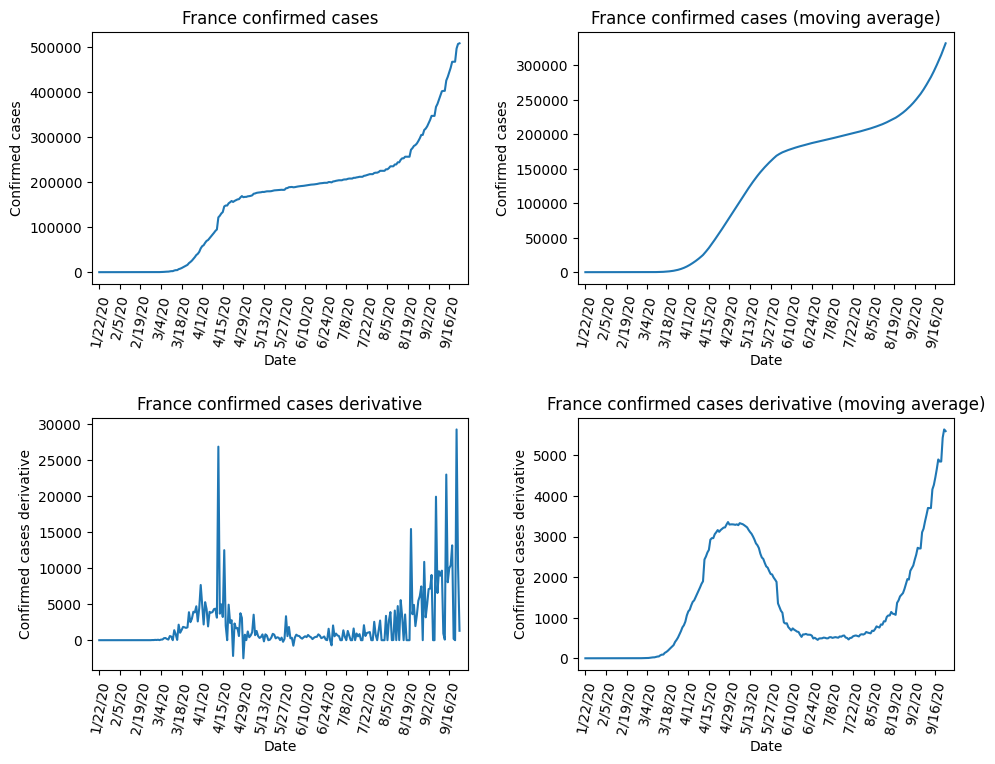
\includegraphics[width=\columnwidth]{img/moving_avg.png}
    \caption{Cas confirmés et dérivée, sans et avec moyenne mobile}
    \label{fig:moving_avg}
\end{figure}

Nous avons ensuite essayé de tronquer les courbes avec la bibliothèque Python \texttt{ruptures} qui
permet de détecter des points singuliers d'une courbe mais nous ne sommes pas parvenus à trouver
des paramètres qui nous donnaient des résultats satisfaisants sur l'ensemble des pays.

Nous avons donc décidé d'utiliser la dérivée de la courbe de cas confirmés pour détecter les changements
de tendance. La dérivée d'une série temporelle est calculée en prenant la différence entre chaque point
de la courbe et le point précédent. Nous localisons le point où la dérivée est maximale pour chaque pays
remontons dans le temps jusqu'à ce que la dérivée soit inférieure à un certain seuil pour tronquer la courbe.
Nous procédons de la même manière de l'autre côté de la courbe en avançant dans le temps jusqu'à ce que la
dérivée soit inférieure à un autre seuil.

Les seuils ont été choisis de manière empirique en observant les résultats produits sur un échantillon de pays
avec des courbes variées. (fig. \ref{fig:clip_full})

Nous avons finalement choisi 5\% comme seuil pour la détection du début de la pandémie et 70\% pour la fin.

\begin{figure}[h]
    \centering
    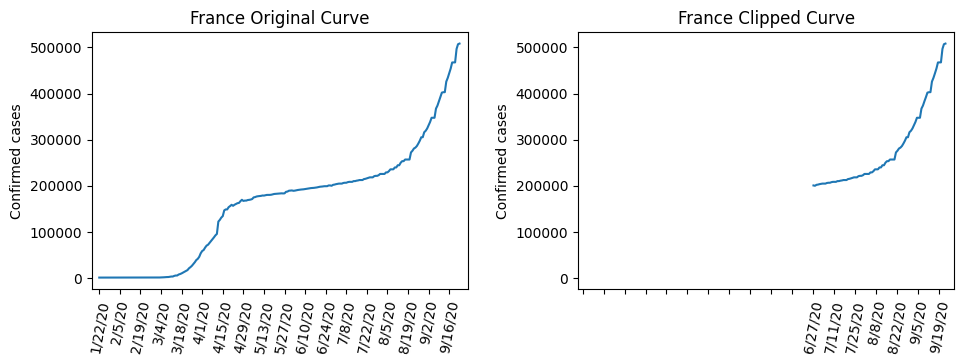
\includegraphics[width=\columnwidth]{img/clip.png}
    \caption{Exemple de troncature, cas de la France}
    \label{fig:clip}
\end{figure}

\subsubsection{Calcul du facteur de propagation}
Il a ensuite fallu extraire des portions de courbes conservées un indicateur de propagation du virus
pour chaque pays. Nous avons testé quatre méthodes différentes :
\begin{itemize}
    \item Régression linéaire
    \item Régression exponentielle
    \item Temps nécessaire pour doubler le nombre de cas
    \item Ratio de reproduction quotidien
\end{itemize}

\noindent\textbf{Régression linéaire} : 

Nous avons ajusté une droite de la forme $y = ax + b$ sur les données de cas confirmés en utilisant
la bibliothèque Python \texttt{scikit-learn} et avons pris le coefficient $a$ comme indicateur de
propagation.

\begin{figure}[h]
    \centering
    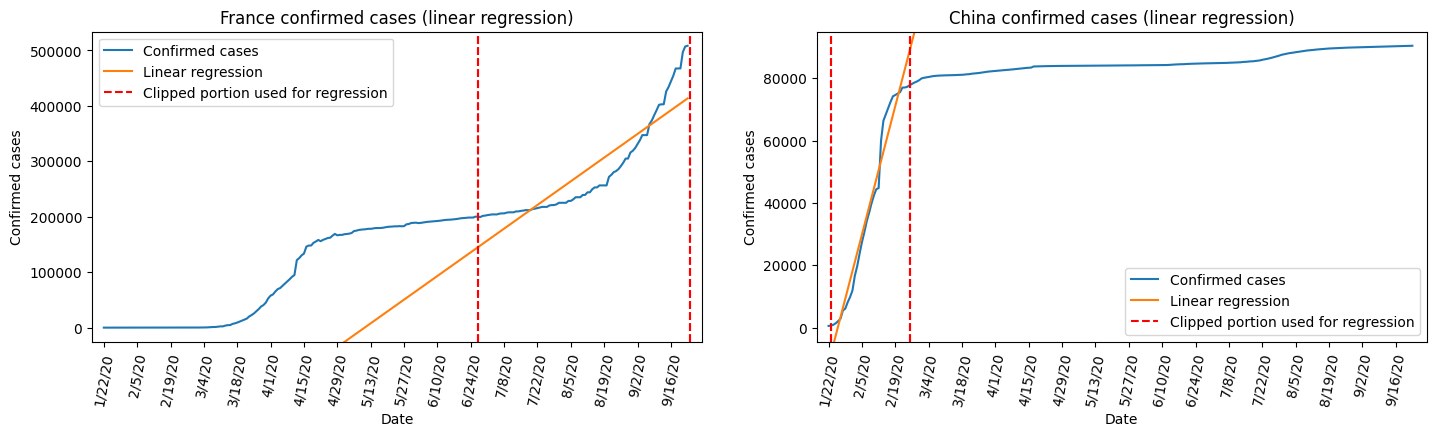
\includegraphics[width=\columnwidth]{img/lin_reg.png}
    \caption{Régression linéaire}

    \label{fig:lin_reg}
\end{figure}

Comme on peut le voir sur la figure \ref{fig:lin_reg}, la régression linéaire ne semble pas être un
bon modèle lorsqu'il s'agit de modéliser la propagation d'un virus. Dans le cas de certains pays, la
droite est proche de la courbe, mais pour la pluaprt ce n'est pas le cas et le coefficient directeur
est sensible à la population totale du pays ce qui n'est pas souhaitable.
\\

\noindent\textbf{Régression exponentielle} :

Nous avons ajusté une courbe de la forme $y = e^{ax+b}$ sur les données de cas confirmés en utilisant
la bibliothèque Python \texttt{scipy} et avons pris le coefficient $a$ comme indicateur de propagation.

Nous nous sommes assurés de translater les courbes tronquées pour que le premier point de la série
aient une ordonnée de 0 avant de faire la régression, et nous avons ensuite translaté la courbe
résultant de la régression pour qu'elle corresponde à la courbe originale.

\begin{figure}[h]
    \centering
    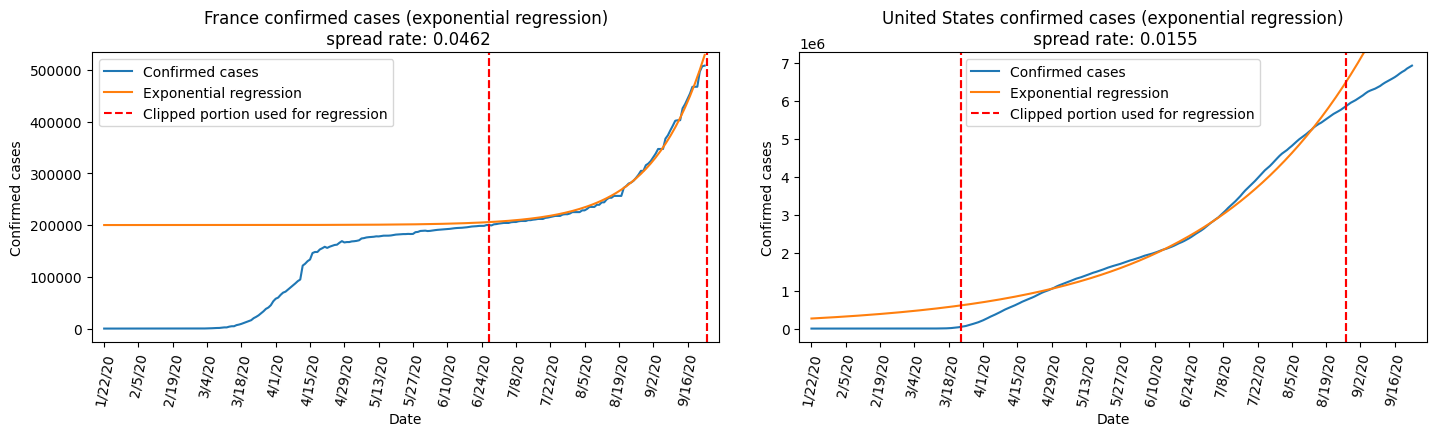
\includegraphics[width=\columnwidth]{img/exp_reg.png}
    \caption{Régression exponentielle}

    \label{fig:exp_reg}
\end{figure}

Comme on peut le voir sur la figure \ref{fig:exp_reg}, la régression exponentielle semble donner
des résultats satisfaisants sur différents types de courbes.

Nous avons appliqué un min-max scaling sur les coefficients obtenus pour chaque pays afin de les
ramener entre 0 et 1 et de pouvoir les comparer.
\\

\noindent\textbf{Temps moyen requis pour doubler le nombre de cas} :

Une autre manière de calculer le taux de propagation est de calculer le temps qu'il faut pour que le nombre
de cas confirmés double. Cette méthode est robuste à la forme de la courbe et facile à calculer mais puisque
nous avons tronqué les séries temporelles à un certain point, l'initialisation ne sera pas la même pour chaque
pays même après translation. Certains pays pourraient déjà avoir gagné un certain élan au début de la série
temporelle tronquée et cela ferait que le temps pour doubler les cas serait plus petit qu'il ne devrait l'être.

Pour éviter cela, nous avons décidé de ne prendre en compte le temps pour doubler les cas qu'à partir
d'une certaine portion de la série temporelle en espérant que le taux de propagation se soit stabilisé.

Ainsi, nous avons choisi de ne considérer que les derniers 75\% de la série temporelle tronquée.

\begin{figure}[h]
    \centering
    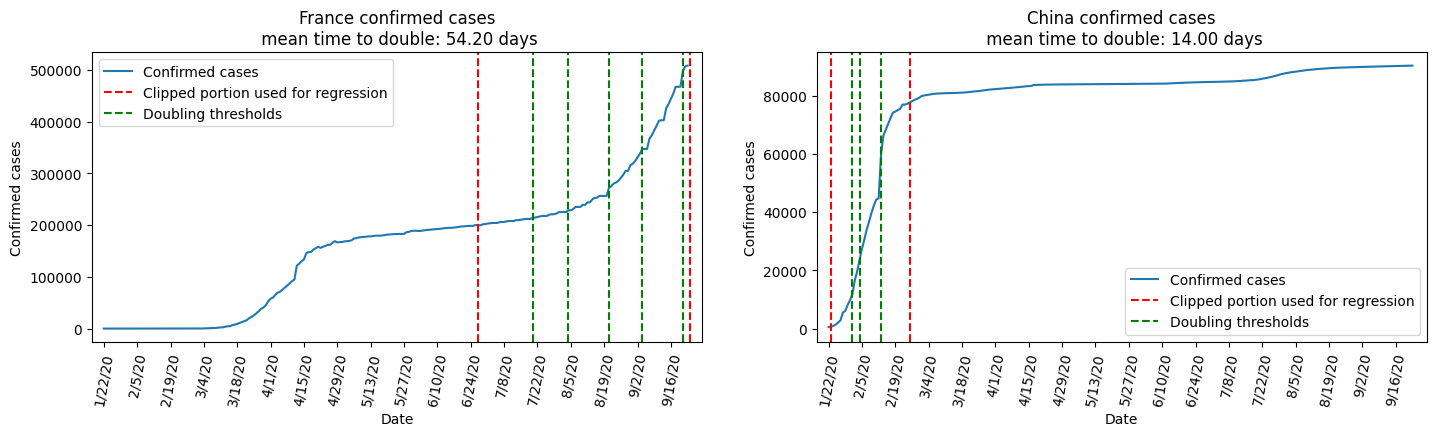
\includegraphics[width=\columnwidth]{img/time_double.png}
    \caption{Temps pour doubler les cas}

    \label{fig:time_double}
\end{figure}

Comme on peut le voir sur la figure \ref{fig:time_double}, notre manipulation a permis de stabiliser
le temps pour doubler les cas pour chaque pays et de minimiser l'impact de l'initialisation.

Pour ramener cet indicateur entre 0 et 1, nous avons utilisé la formule suivante :
$$v' = \frac{v_{max}-v}{v_{max}}$$ où $v_{max}$ est le temps pour doubler les cas le plus grand parmi
tous les pays.
\\

\noindent\textbf{Ratio de reproduction quotidien} :

Cette méthode consiste à calculer l'augmentation relative moyenne du nombre de cas confirmés par jour
sur la période considérée. C'est une méthode simple et intuitive qui semble fonctionner correctement.

La formule utilisée est la suivante :
$$v = \frac{1}{n-1} \sum_{i=1}^{n-1} \frac{c_{i+1} - c_i}{c_i}$$ où $c_i$ est le nombre de cas confirmés
au jour $i$ et $n$ est le nombre de jours considérés.

Voici les valeurs que l'on obtient pour quelques pays :
\begin{table}[h]
    \centering
    \begin{tabular}{|c|c|}
        \hline
        Pays & Ratio de reproduction quotidien \\
        \hline
        France & 0.052 \\
        United Kingdom & 0.042 \\
        United States & 0.015 \\
        China & 0.098 \\
        Russia & 0.031 \\
        Ethiopia & 0.035 \\
        Afghanistan & 0.052 \\
        \hline
    \end{tabular}
\end{table}

À nouveau, un min-max scaling a été appliqué pour ramener les valeurs entre 0 et 1.
\\

\noindent\textbf{Comparaison des méthodes} :

Afin de comparer les différentes méthodes, nous avons affiché les positions de quelques
pays pour chacune d'entre elles. (fig. \ref{fig:spread_comp})

\begin{figure}[h]
    \centering
    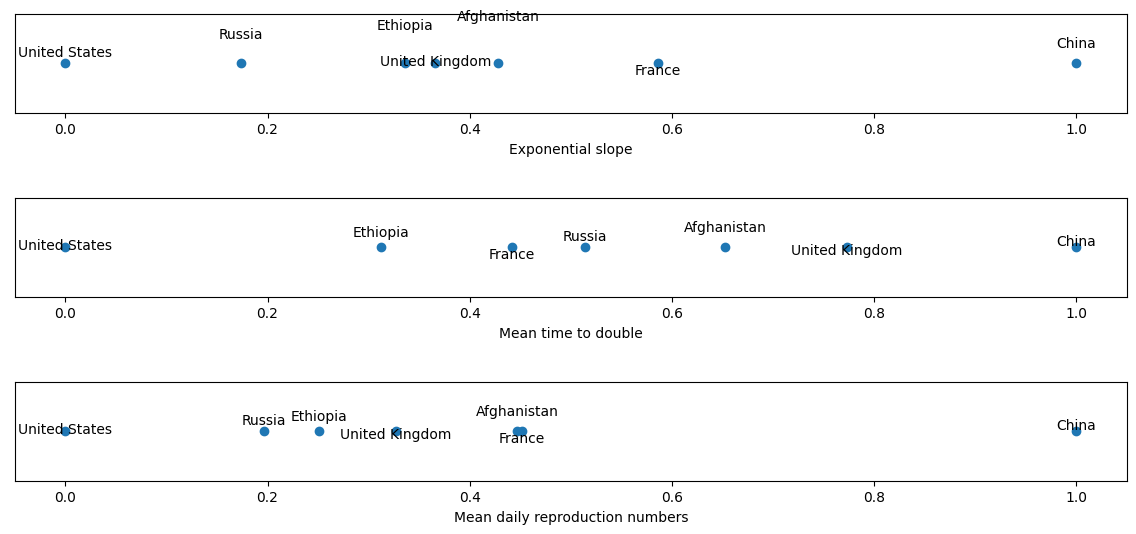
\includegraphics[width=\columnwidth]{img/spread_comp.png}
    \caption{Comparaison des méthodes de calcul de la propagation}

    \label{fig:spread_comp}
\end{figure}

On constate notamment que le temps moyen pour doubler les cas présente un classement assez
différent des deux autres méthodes.

Après avoir comparé les résultats de la régression exponentielle et du ratio de reproduction
quotidien entre eux et avec les courbes, nous avons décidé de poursuivre notre étude en
utilisant le coefficient de la régression exponentielle comme indicateur de propagation.

\subsection{Résultats et interprétation}
\textit{TODO : spread/position, spread/urban population, spread/climate et comparaison entre
spread et mortality rate}

\subsection{Applications concrètes}
\textit{TODO : Meilleure gestion des pandémies, meilleure compréhension des facteurs
influant sur la propagation du virus.}
\subsection{Limites}
Nous avons été limités par la qualité des données disponibles. En effet, certaines données
ne sont disponibles que par pays et d'autres pour des points du globe. Nous avons donc dû
faire des approximations pour pouvoir les utiliser. Ce point pose notamment problème pour
la classification climatique de Köppen-Geiger qui est disponible pour des points du globe et
peut différer d'une région à l'autre d'un même pays. Également, les données de COVID-19
ne sont disponibles qu'à l'échelle des pays ou de grandes régions, ce qui ne nous permet
pas de faire des analyses plus fines quant aux différences d'urbanisation au sein des pays.

\subsection{Conclusion}
\textit{TODO : Répondre à la problématique, donner des pistes pour des études futures.}

\bibliographystyle{plain}
\bibliography{bibliography}

\newpage

\section{Annexes}
\begin{figure}[h]
    \centering
    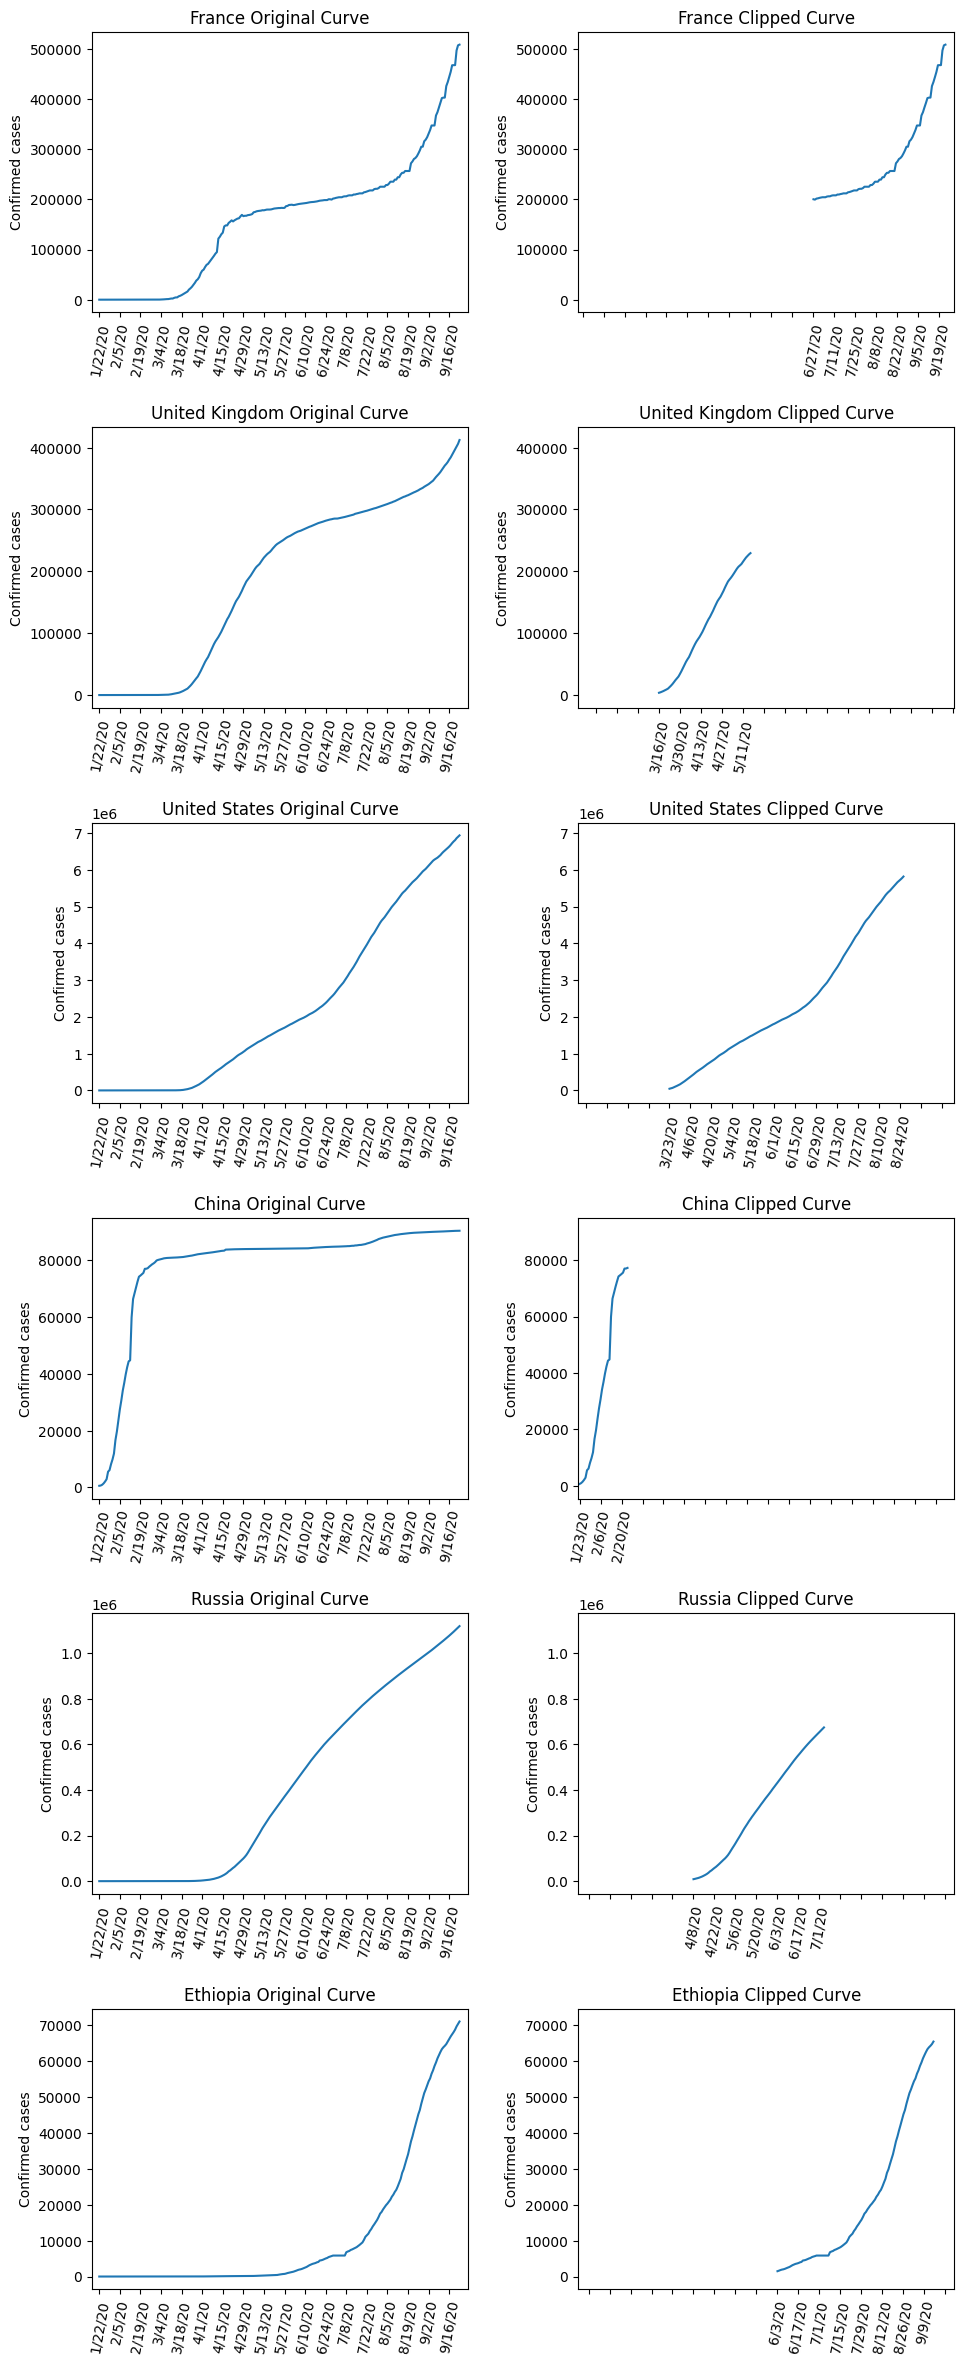
\includegraphics[width=8cm]{img/clip_full.png}
    \caption{Troncature des courbes de cas confirmés}
    \label{fig:clip_full}
\end{figure}

\end{document}